\subsection{Mikrofone}
    \subsubsection{Richtcharakteristiken}
Die Richtcharakteristik gibt an, aus welcher Richtung und wie stark bzw. empfindlich ein Mikro auftreffende Schallwellen aufnimmt. Je nachdem welche Richtcharakteristik ein Mikrofon hat, ist es aus bestimmten Richtungen empfindlicher für Schall als andere Mikrofone. Mikrofone unterscheiden sich in diesem Punkt daher gar nicht so viel von dem menschlichen Gehör – auch wir haben unterschiedliche Arten zu hören und Informationen aufzunehmen: Der Schall von vorne wird lauter empfangen als der Schall von hinten (Abschattungseffekte durch Ohrmuschel).\cite{BeyerRichtchar}
\begin{center}
    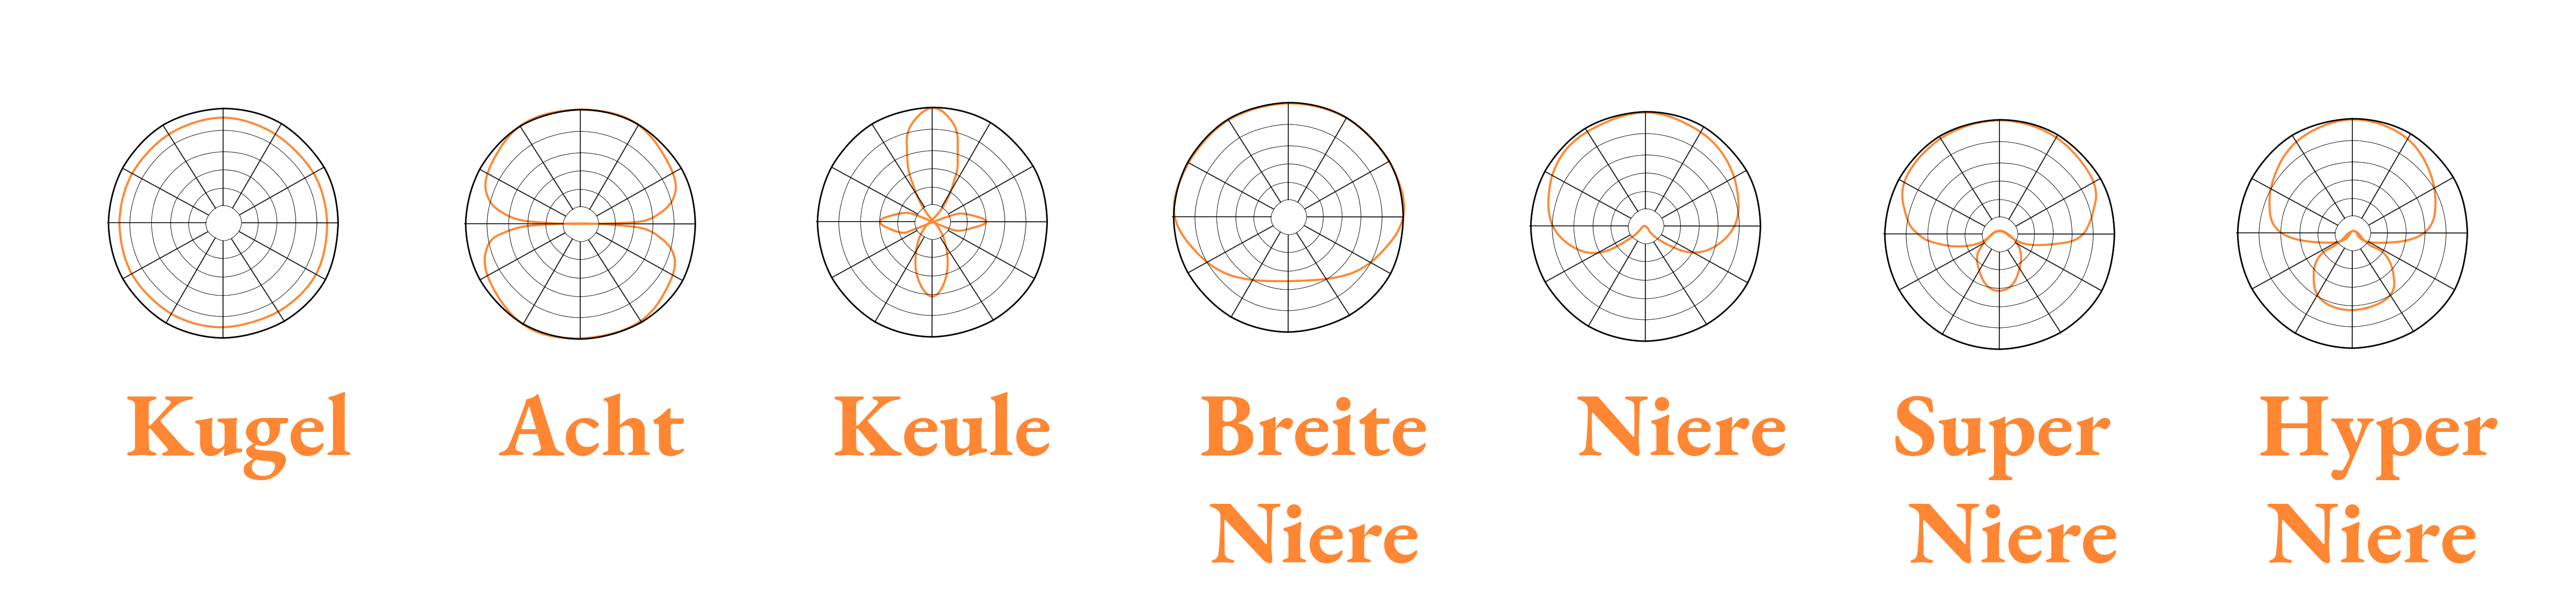
\includegraphics[width=1\textwidth]{Bilder/Medientechnik/Mikrocharakteristik.png}
\end{center}

Polardiagramm = Darstellung der Charakteristik in einer 2-Dimensionalen Ebene, zum Vergleich hier eine realistischere 3 Dimensionale Abbildung. Zu beachten ist das man mit dieser nicht gut Arbeiten kann.

\begin{center}
    \includegraphics[width=0.3\textwidth]{Bilder/Medientechnik/Mic_Niere.png}\hspace{3mm}\includegraphics[width=0.3\textwidth]{Bilder/Medientechnik/Mic_Keule.png}\hspace{3mm}\includegraphics[width=0.3\textwidth]{Bilder/Medientechnik/Mic_Acht.png}\\
    Niere \hspace{3.2cm} Keule \hspace{3.2cm} Acht
\end{center}

\paragraph{Die wichtigen 3 Charakteristiken}~\\

\begin{wrapfigure}{hr}{4cm}\vspace{-1cm}
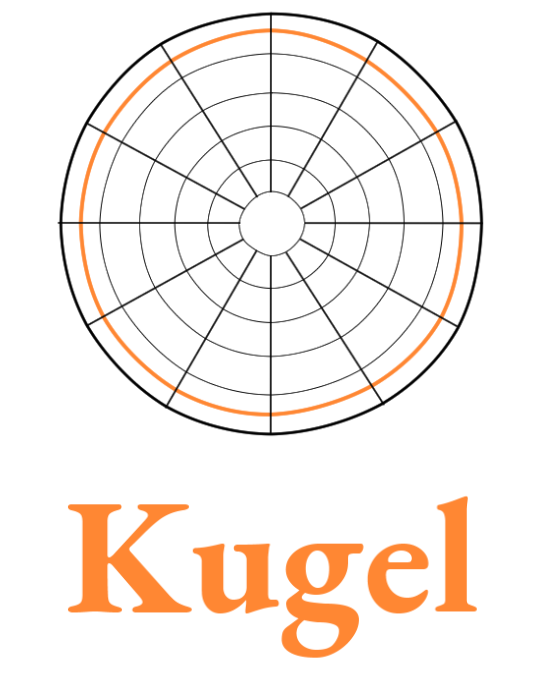
\includegraphics[height=4cm]{Bilder/Medientechnik/Mikrocharakteristik_Kugel.png}
\end{wrapfigure}
 \textbf{Kugelcharakteristik} Mikrofone, die diese Richtcharakteristik aufweisen, nehmen Schallwellen gleichermaßen aus allen Richtungen, also omnidirektional, auf. Das dazugehörige Polardiagramm zeigt aus diesem Grund einen Kreis. Diese Mikrofone eignen sich besonders gut, um mehrere Menschen gleichzeitig aufzunehmen, die rundherum um das Mikro stehen. Sie werden daher oft bei Film-, Video- oder redaktionellen Hörfunkprojekten eingesetzt. Dadurch, dass Mikrofone mit Kugelcharakteristik alles um sich herum aufzeichnen, sind sie allerdings verstärkt rückkopplungsanfällig und für sehr laute und unruhige Umgebungen eher ungeeignet.\\

\begin{wrapfigure}{hr}{4cm}\vspace{-1cm}
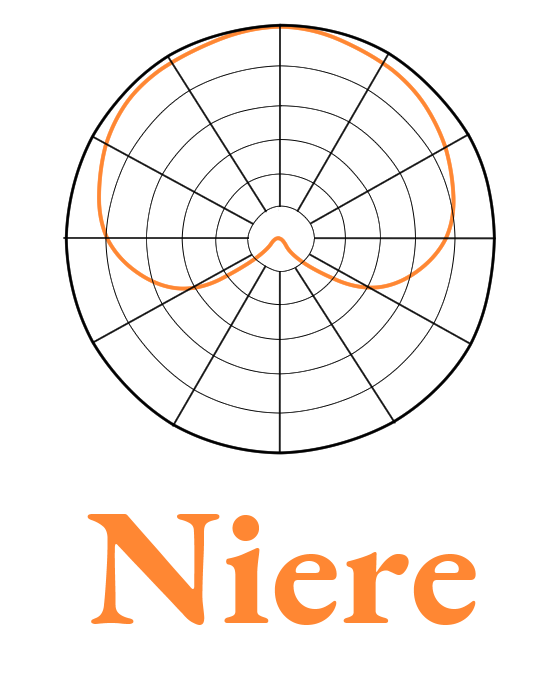
\includegraphics[height=4cm]{Bilder/Medientechnik/Mikrocharakteristik_Niere.png}
\end{wrapfigure}
 \textbf{Nierecharakteristik} Die klassische Niere kann als eine zu gleichen Teilen zusammengesetzte Mischung aus einer Kugel und einer Acht verstanden werden. Mikrofone mit Nierencharakteristik nehmen vorrangig Schall von vorne auf und blenden Töne von hinten – also aus 180° – aus. Seitliche Schallwellen werden von vorne nach hinten zunehmend abgeschwächt aufgezeichnet. Der entscheidende Vorteil dieser Richtcharakteristik ist, dass diese Mikrofone weniger rückkopplungsanfällig sind wie beispielsweise ein Kugelmikrofon aber dennoch durch den breiten Aufnahmewinkel auf der Vorderseite eine weniger exakte Ausrichtung auf die Schallquelle verzeihen.\\~\\Eine recht komplexe Angelegenheit, es ist eine Mischung aus einer Acht und einer Kugel. Hierfür werden 2 Mikrofone benötigt um 1nes Herzustellen.
Meist wird eine Kugel genommen und ein Stück Schaumstoff mit Schallverlangsamenden Eigenschaften benutzt um es von hinten Auszugleichen und von vorne her gut zu verwenden.\\

 \begin{wrapfigure}{hr}{4cm}\vspace{-1cm}
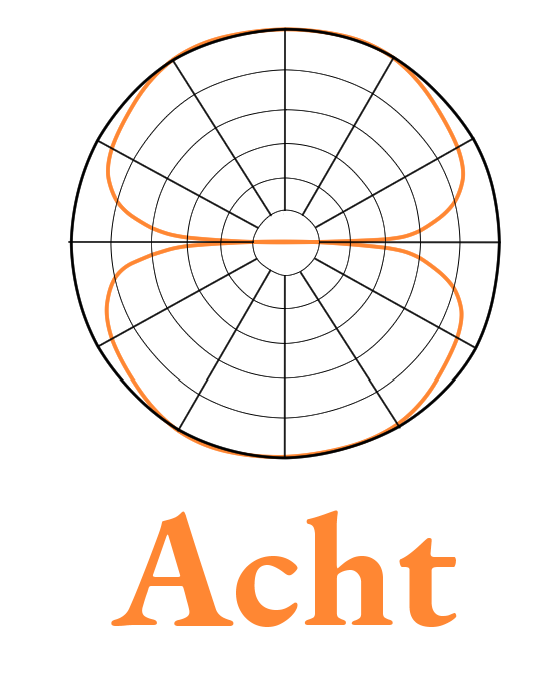
\includegraphics[height=4cm]{Bilder/Medientechnik/Mikrocharakteristik_Acht.png}
\end{wrapfigure}
 \textbf{Achtercharakteristik} In diesem Fall nimmt das Mikrofon sehr viel Schall von vorne und von hinten auf. Seitlich zeichnet es hingegen nahezu keine Schallwellen auf – die Hauptauslöschung liegt demnach bei 90° bzw. 270°. Die Achtercharakteristik ist vor allem bei Bändchenmikrofonen zu finden, was hauptsächlich an ihrer besonderen Bauform liegt. Vorteilhaft ist, dass seitliche Störgeräusche stark reduziert werden.\\ Hier ist es noch wichtig zu bemerken das sich identischer Schall von den Seiten gegenseitig auslöscht.

 \paragraph{Beispielmikrofone und Zugehörige Hardware}~\\


\begin{center}
    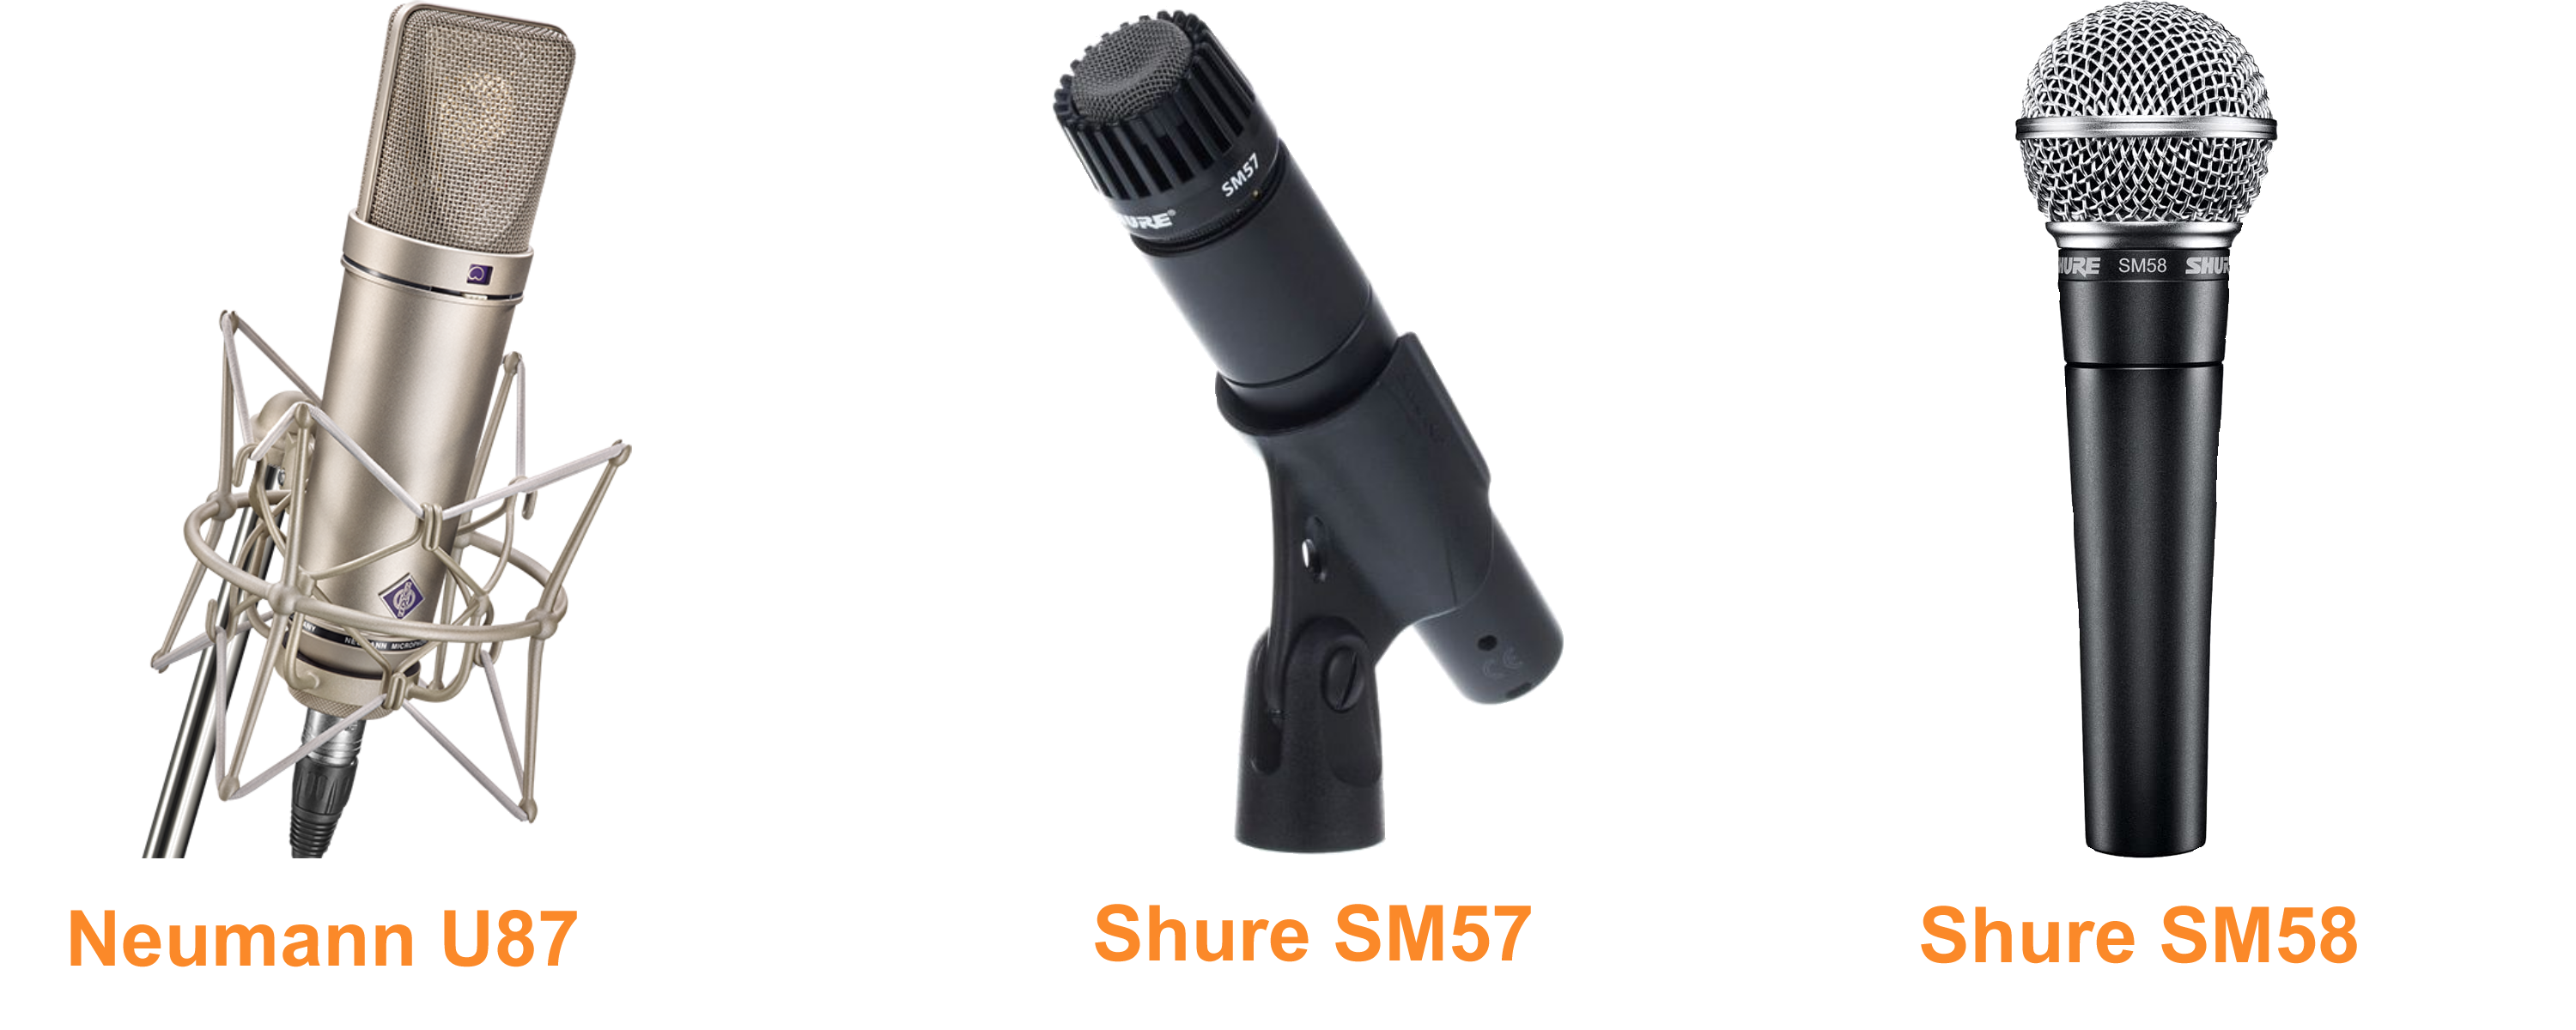
\includegraphics[width=1\textwidth]{Bilder/Medientechnik/U87Sm57Sm58.png}\\
\end{center}
    \textbf{\href{https://www.neumann.com/de-de/produkte/microphones/u-87-ai/}{Neumann U 87}}\cite{NeumannU87:online} ist so das Standart Studiomikrofon\\
    \textbf{\href{https://www.shure.com/de-DE/produkte/mikrofone/sm57?variant=SM57-LCE}{Shure SM 57}} \cite{ShureSM57:online} besitzt einen geringen Kapselabstand\\
    \textbf{\href{https://www.shure.com/de-DE/produkte/mikrofone/sm58?variant=SM58-LCE&utm_source=google&utm_medium=cpc&utm_campaign=26-ao-mu-de-de-sl-jul24-conv-mco-brand&utm_term=sm58-prosp&utm_content=&vdr=sl&sfid=ao-mu&gad_source=1&gclid=CjwKCAjw5Ky1BhAgEiwA5jGujgRsHkHIH6hyjmigzxoFEGLfoI3Nk0UQ5E8CJrlKrQM2YeIal77KjRoCKhEQAvD_BwE}{Shure SM 58}} \cite{SM58:online} gilt so als das \href{ https://www.youtube.com/watch?v=Lz1_l_HJlPA&ab_channel=MusikersajtenStudio}{unzerstörbare} Gesangsmikrofon.\\
    \textbf{\href{https://www.k-m.de}{K\&M (König und Meyer)}} ist der Standart bei Stativen.  \newpage